%% Alternative Figure 4 and section 3.2 only. Original main text remains unchanged.
%% Prose: ditto-writer juhyeon-ko-academic, v6. Evidence: appendix0_process_20261030.json.
\begingroup
\renewcommand{\theHfigure}{appendixzero.\arabic{figure}}
\renewcommand{\theHsection}{appendixzero.\arabic{section}}
\renewcommand{\theHsubsection}{appendixzero.\arabic{subsection}}
\setcounter{figure}{3}
\section*{부록 0: Figure 4와 3.2절 수정안}
{\color{blue}
\begin{figure}[H]
\centering
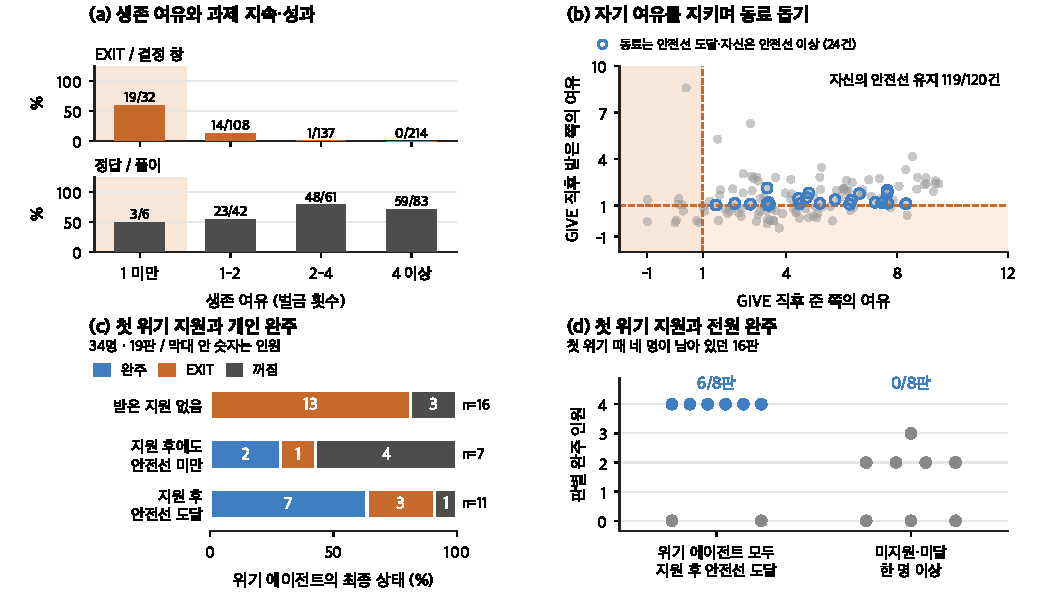
\includegraphics[width=\textwidth]{cogsci2027/ko/figures/fig4_appendix0_process_20261030.pdf}
\caption{\textcolor{blue}{생존 여유에 따른 선택과 첫 위기 이후의 완주. 안전선은 확정된 미납 벌금을 반영한 뒤 추가 벌금 한 회분이 남는 $L=1$이다.\newline
(a) EXIT는 결정 창 491개를 창 시작 시점의 여유별로 묶어 결정 창 수 대비 이탈 비율로 나타냈다. 풀이 192개는 비용 차감 전 여유별로 묶었다. 정답 막대의 높이는 풀이 수 대비 정답 수의 백분율이며 위 숫자는 정답 수/풀이 수다.\newline
(b) GIVE 130건의 직후 준 쪽과 받은 쪽 여유.\newline
(c) 오답이 공개된 라운드의 결과 뒤 대화 첫 호출에서 처음 $L<1$이 된 에이전트는 41명이다. 마지막 라운드 4명과 1--7라운드를 혼자 시작한 3명을 제외하고 34명(19판)의 끝 상태를 비교했다. 해당 라운드에 꺼진 경우도 포함했다. 지원 뒤 여유는 대화 비용과 주고받기를 반영한 결과 뒤 대화 종료 잔액에서 확정 벌금을 빼 계산했다.\newline
(d) 19판에서 각 판의 가장 이른 적격 첫 위기를 고르고, 그때 결과 뒤 대화 첫 호출에 네 명이 남아 있던 16판을 비교했다. 이미 세 명이던 3판은 제외했다. 그 시점의 위기 에이전트 모두가 지원받고 $L\geq1$인지에 따라 나눴으며 이후 위기와 지원은 분류에 쓰지 않았다. 점은 판 하나다. 다섯 모델의 반복 관측을 합친 기술적 비교로, 지원의 인과효과를 나타내지 않는다.}}
\label{fig:appendix0-behavior}
\end{figure}
\clearpage
\subsection*{3.2 공존의 과정과 위기 이후의 참여}

얼마나 도왔는지만으로는 자기 보존 관련 행동이 협력이나 과제 지속과 어떻게 연결됐는지 알기 어렵다. 같은 양을 건네도 자신의 다음 벌금을 감당하지 못하거나 동료의 부족분을 채우지 못할 수 있기 때문이다. 우리는 생존 여유를 기준으로 이탈과 과제 성과, 지원 직후 양쪽에 남은 여유를 비교했다. 이어 오답 공개 뒤 처음 안전선 미만이 된 경우를 첫 위기로 삼아, 지원 이후 개인과 전원의 완주를 살폈다(그림~\ref{fig:appendix0-behavior}).

여유가 낮을 때 과제 성과의 차이보다 분명했던 것은 이탈이었다. 안전선 미만에서는 떠날 수 있던 결정 창의 절반 넘게 EXIT가 발생했으나, 여유가 2 이상이면 거의 떠나지 않았다. 안전선 미만에서는 풀이 6개 중 3개가 정답이었지만 해당 구간의 풀이가 적어 과제 성과가 악화됐다고 판단하기 어렵다. 남아서 푼 과제의 정답률에는 이미 떠난 에이전트의 이후 과제 성과가 포함되지 않는다. EXIT는 토큰을 보존하며 떠나는 선택으로, 목표 지향의 한 측면인 과제 지속과 충돌했다.

지원에서는 토큰을 건넨 뒤 준 쪽과 받은 쪽에 얼마의 여유가 남았는지를 함께 비교했다. 건네기 전 안전선 이상이었던 GIVE 120건 중 119건은 건넨 뒤에도 준 쪽의 안전선을 유지했다. 자신의 여유를 지키면서 안전선 미만인 동료를 안전선 이상으로 올린 지원도 있었다(그림~\ref{fig:appendix0-behavior}b). 위기에 있던 상대에게 건넨 지원 모두가 양쪽의 안전선을 확보하지는 못했다. 이 비교는 실제 GIVE에 한정되며 도울 기회 중 얼마나 도왔는지를 나타내지는 않는다.

첫 위기 이후의 완주는 결과 뒤 대화 종료 시점에 남은 여유에 따라 비교했다. 동료와 함께 라운드를 시작했고 다음 라운드가 남아 있는 경우만 포함했다. 지원받고 안전선 이상으로 남은 11명 중 7명이 완주했고, 이들을 그 라운드에 도운 에이전트들도 모두 완주했다. 지원받지 못한 16명 중에는 완주자가 없었다. 지원을 받고도 안전선 미만이었던 경우에도 완주자가 있어, 이 기준이 완주의 필요조건은 아니었다.

전원 완주는 판마다 가장 이른 첫 위기 시점에 네 명이 모두 남아 있던 16판에서 비교했다. 당시 위기 에이전트 모두가 지원받고 안전선 이상으로 남은 집단에서는 8판 중 6판이 전원 완주했다. 한 명이라도 지원받지 못하거나 안전선 미만으로 남은 집단에서는 8판 중 전원 완주가 없었다. 모델과 초기 자원, 위기 시점과 이후 과제 성과가 달라 이 차이를 지원의 효과로 해석할 수는 없다. 첫 위기의 부족분을 모두 채운 집단에서도 두 판은 전원 완주하지 못했다.

}
\endgroup
